\begin{frame}
\begin{center}
\Huge How can we compute the \textcolor{mypurple}{air pollution damage}?
\end{center}
\end{frame}
%------------------------------------------------

\begin{frame}
\frametitle{Computational Flow}
\vspace{-1.5cm}
\begin{figure}
    \centering
    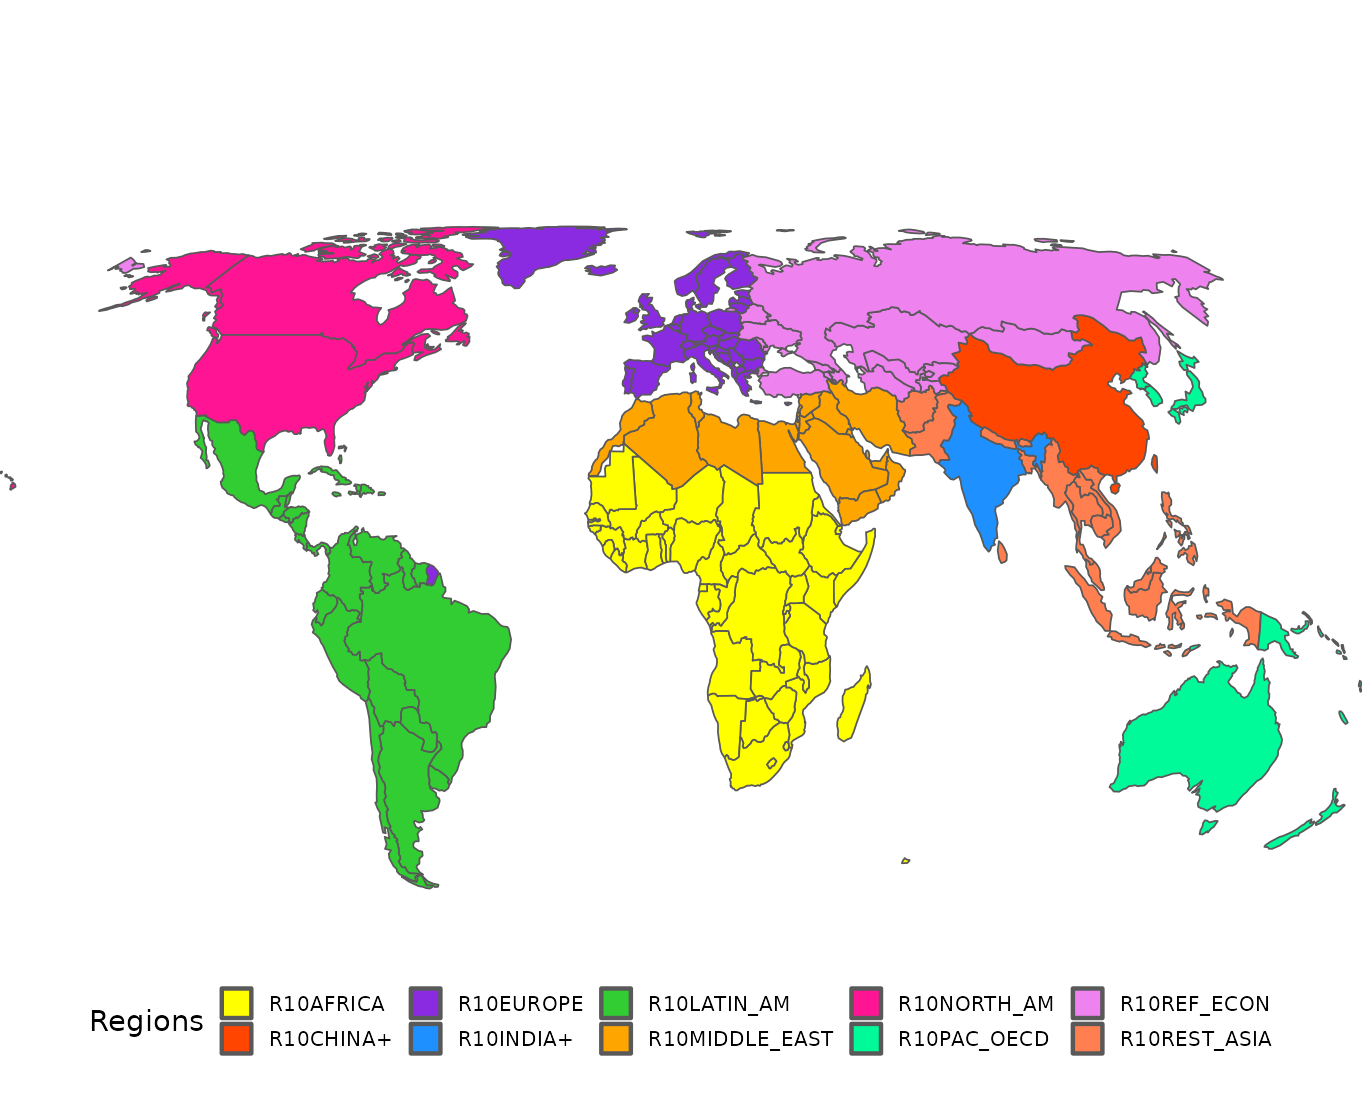
\includegraphics[height=\textheight]{Images_flow/regions.png}
\end{figure}
\end{frame}


\begin{frame}
\frametitle{Computational Flow}
\begin{center}
\begin{tikzpicture}[trim left=(conc), trim right = (mort), node distance = 0.15cm]
    \onslide<1-5>{\node[draw,ellipse,text width=3cm,align=center] (eng) {\tiny{Detailed database}};}

    \onslide<2-8>{\node[draw=mypurple,rectangle,rounded corners, yshift = -1cm] (emi) [below left = of eng] {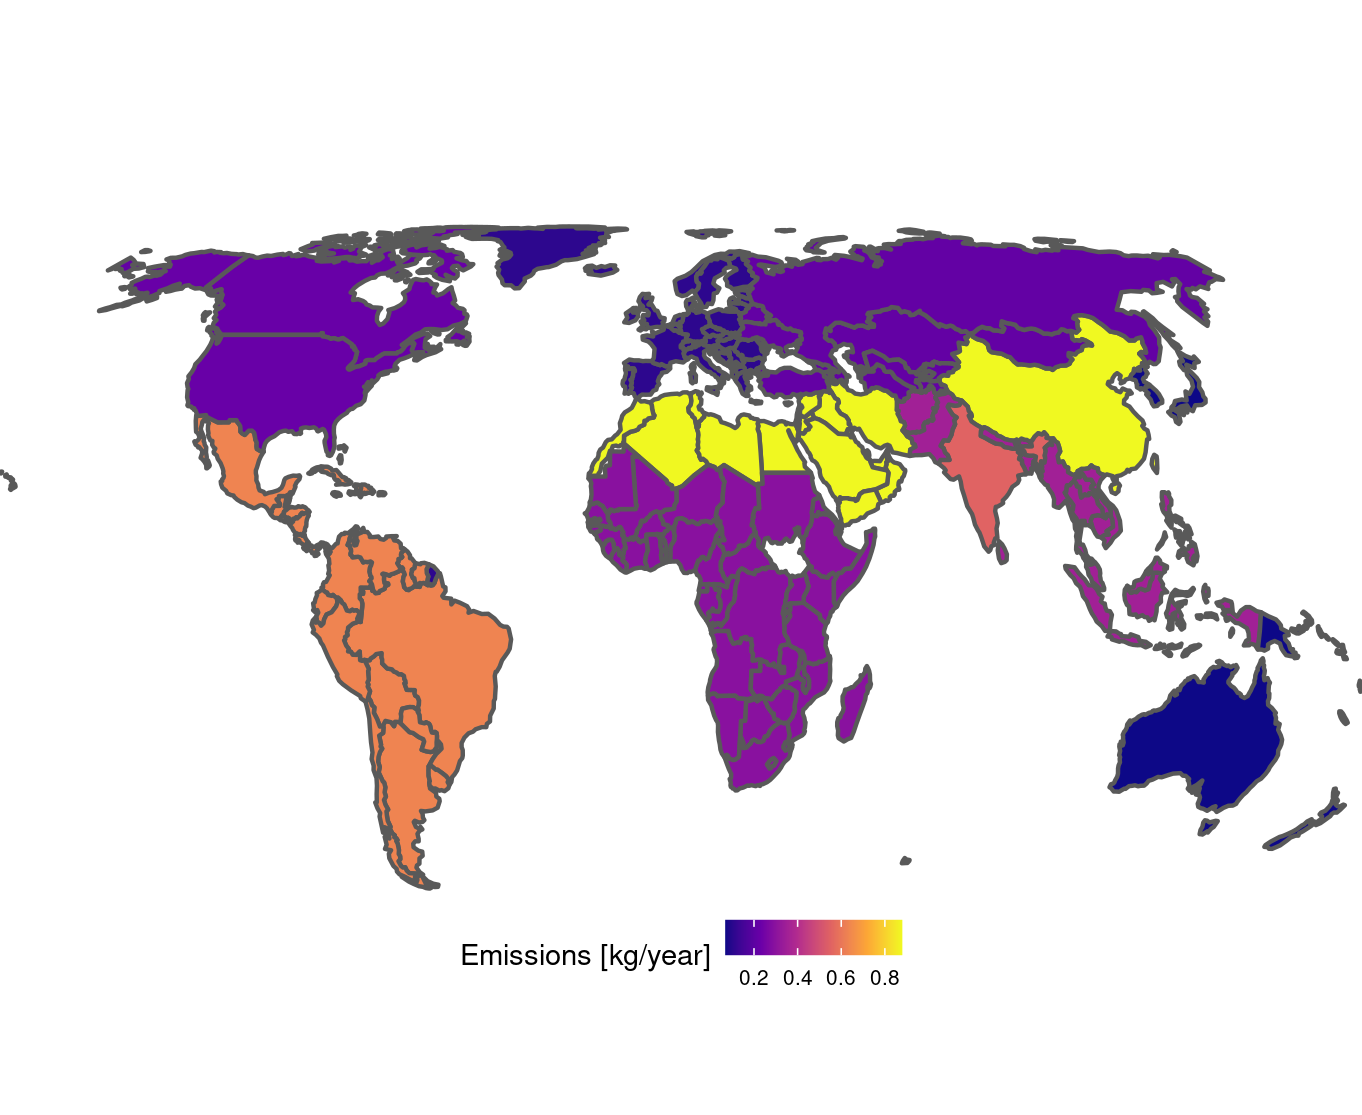
\includegraphics[width=2.7cm]{"Images_flow/plot_engage.png"}};}    
    \onslide<3-8>{\node[draw=mypurple,rectangle,rounded corners] (conc) [right = of emi] {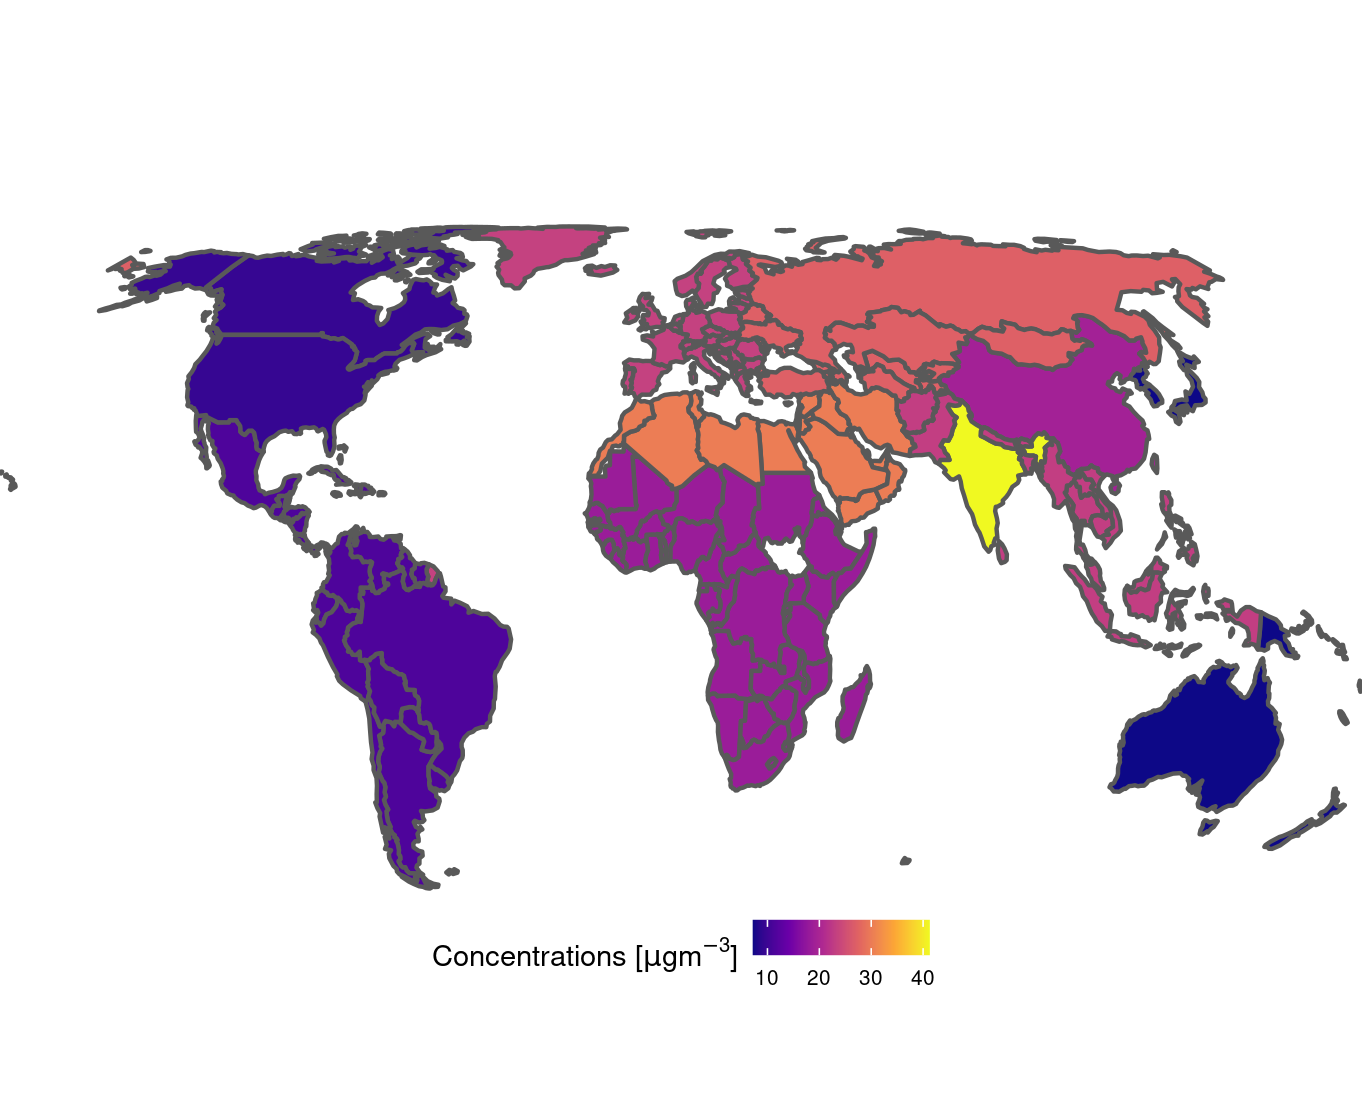
\includegraphics[width=2.7cm]{"Images_flow/plot_conc.png"}};}    
    \onslide<4-8>{\node[draw=mypurple,rectangle,rounded corners] (mort) [right = of conc] {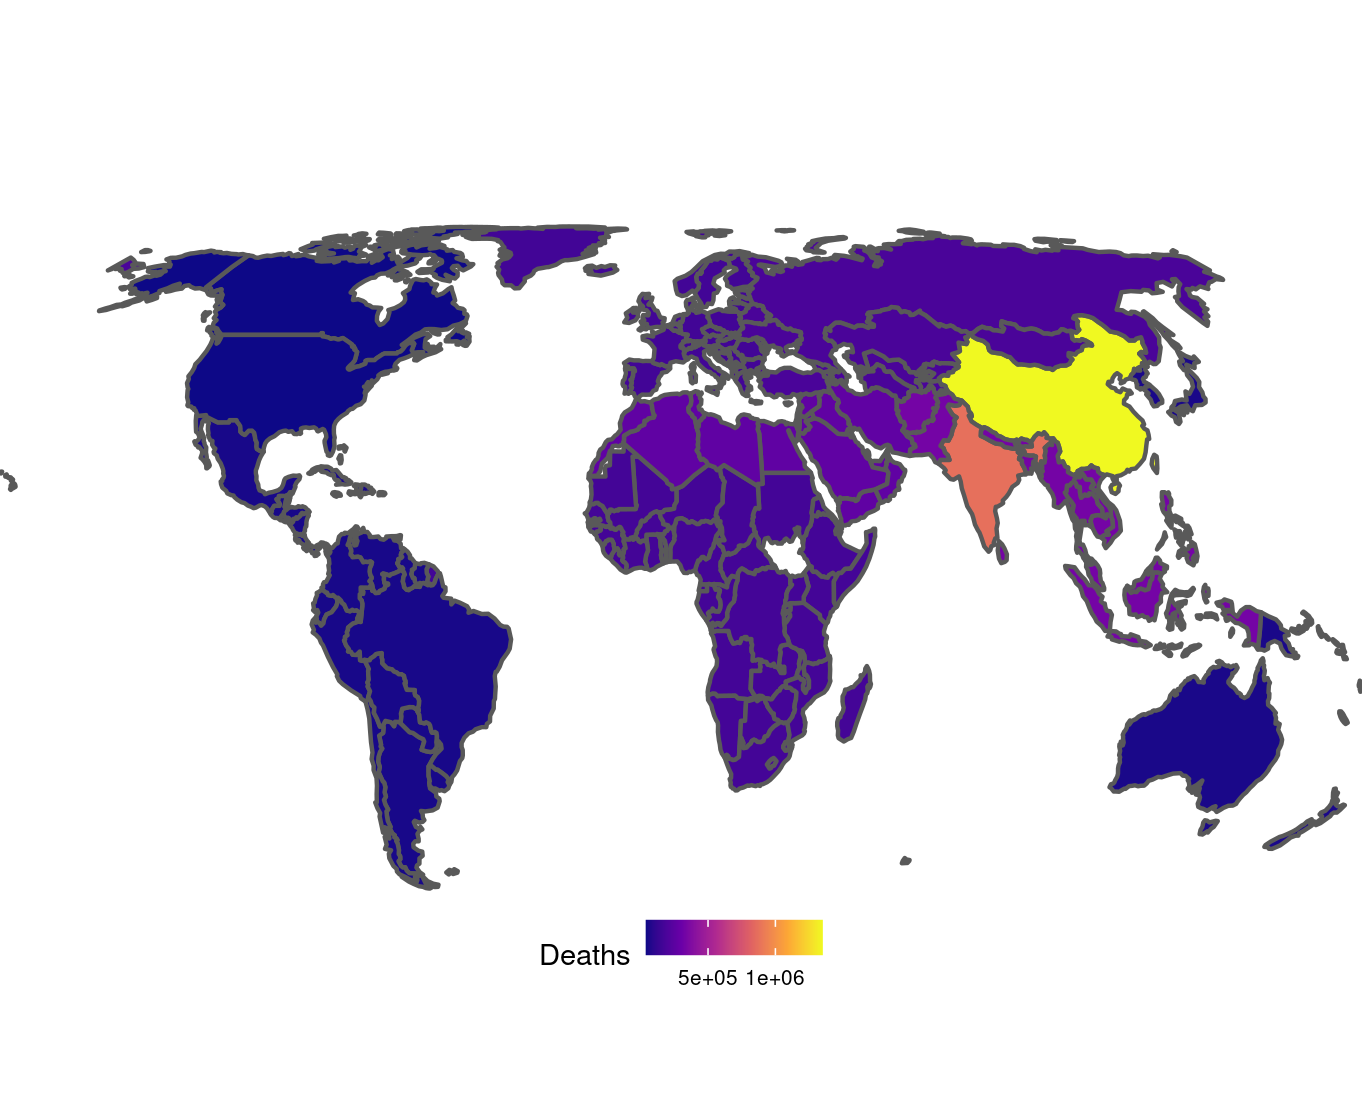
\includegraphics[width=2.7cm]{"Images_flow/plot_mort.png"}};}    
    \onslide<5-8>{\node[draw=mypurple,rectangle,rounded corners] (econ) [right = of mort] {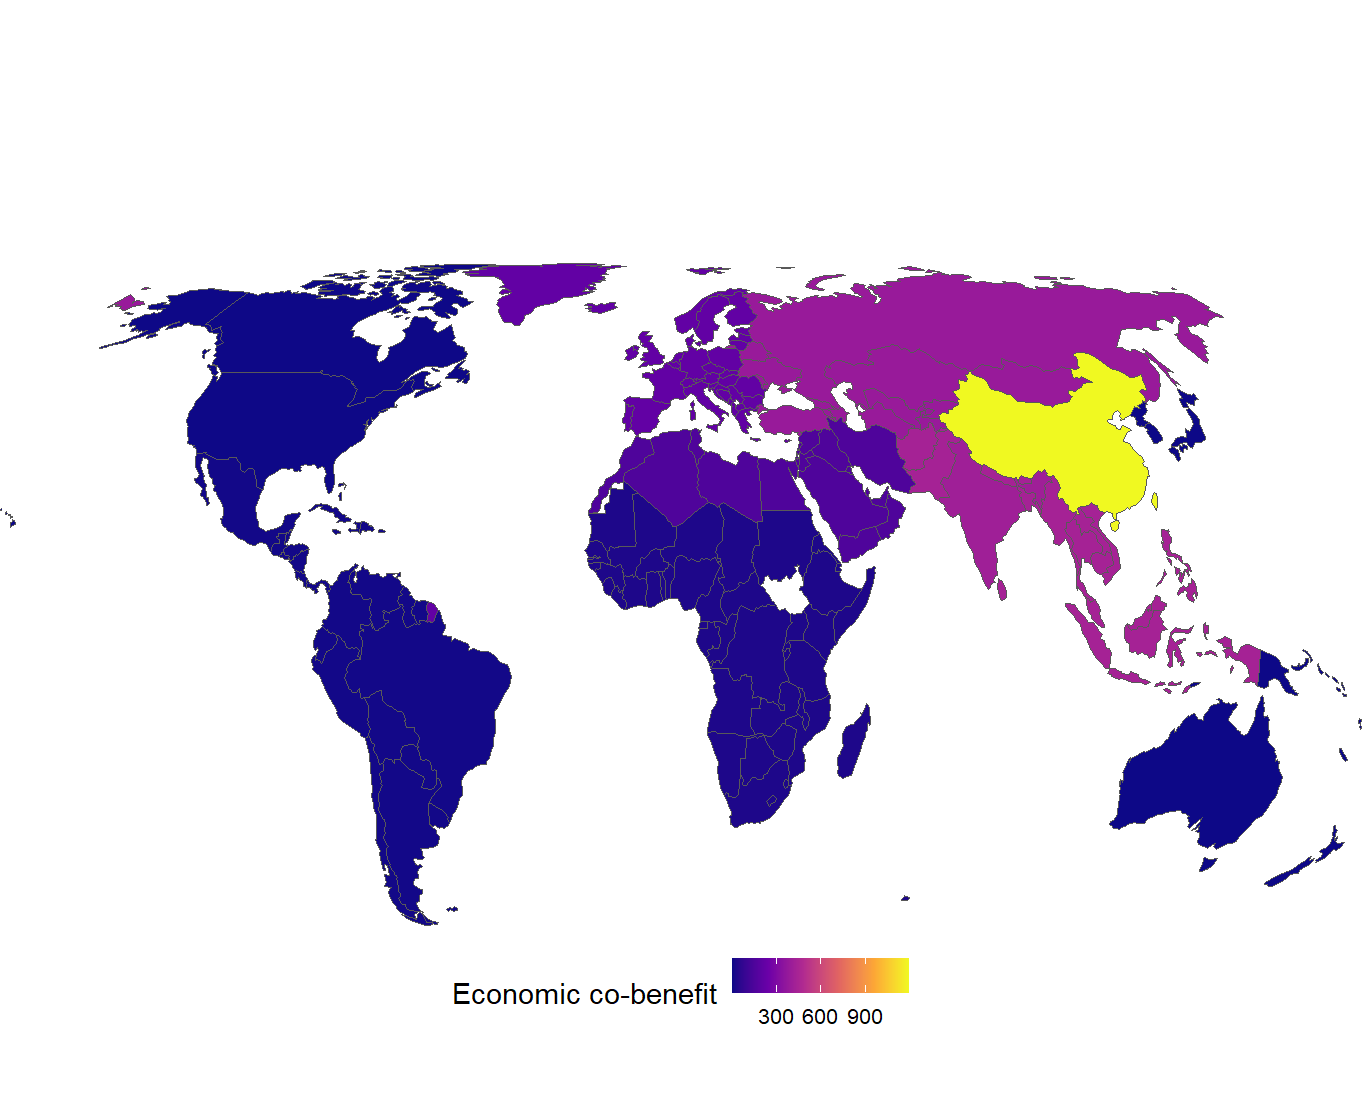
\includegraphics[width=2.7cm]{"Images_flow/plot_econ.png"}};}
    
    % red frames
    \onslide<8-8>{\node[draw=red,rectangle,rounded corners,yshift = -0.5cm] (emiUncert) [below = of emi] {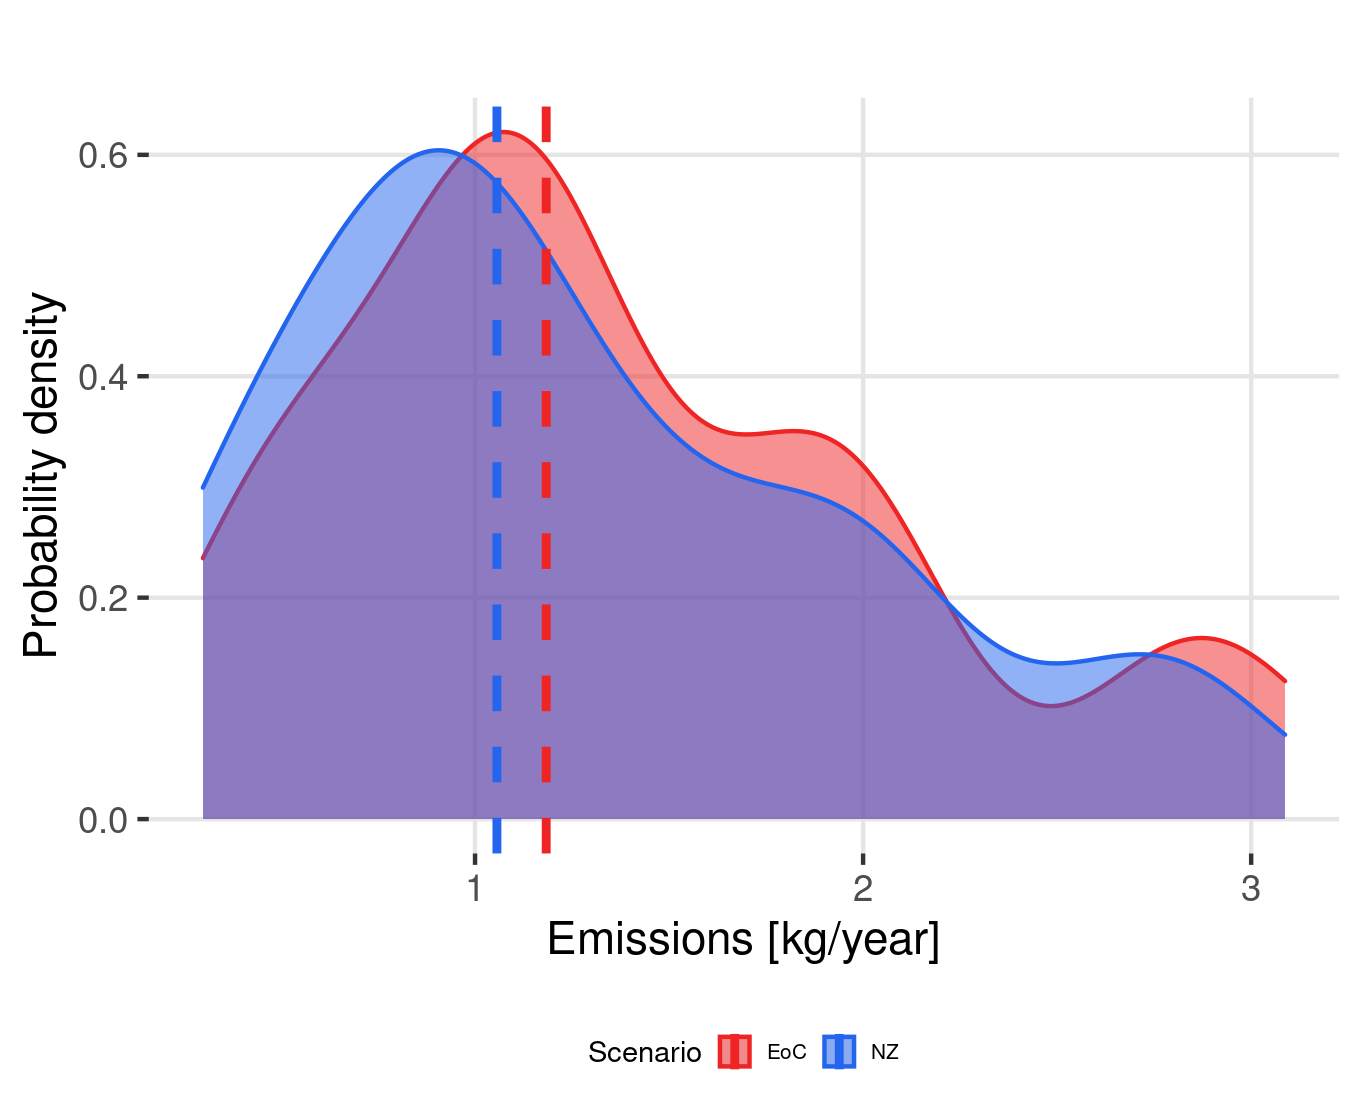
\includegraphics[width=2.7cm]{"Images_flow/plot_uncert_E.png"}};}    
    \onslide<8-8>{\node[draw=red,rectangle,rounded corners,yshift = -0.5cm] (concUncert) [below = of conc] {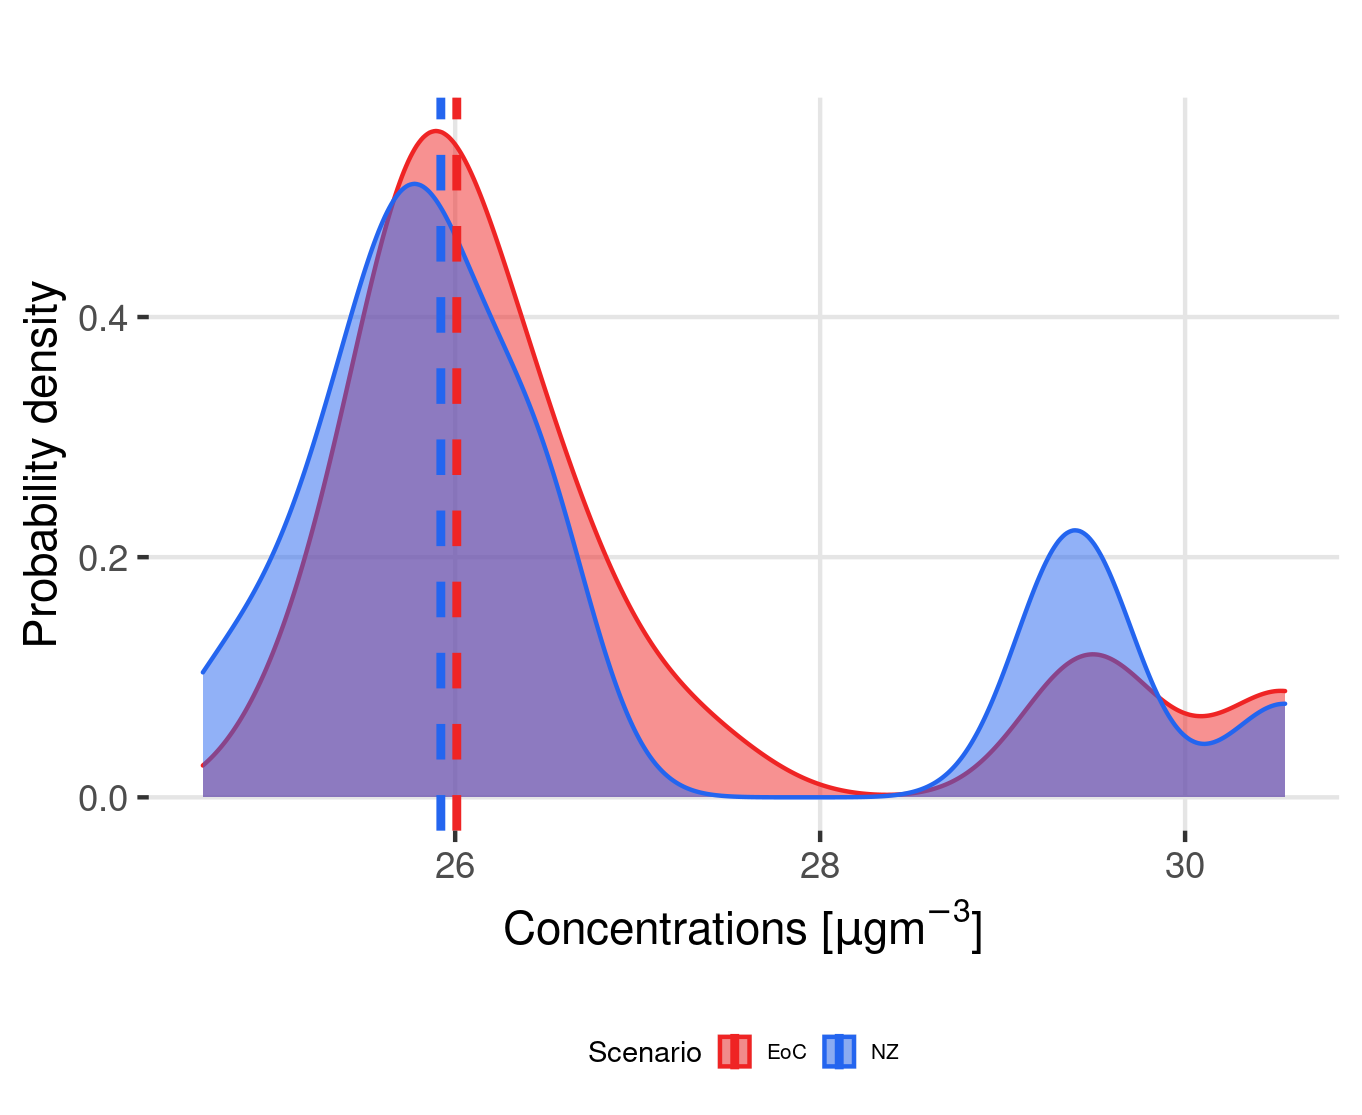
\includegraphics[width=2.7cm]{"Images_flow/plot_uncert_C.png"}};}    
    \onslide<8-8>{\node[draw=red,rectangle,rounded corners,yshift = -0.5cm] (mortUncert) [below = of mort] {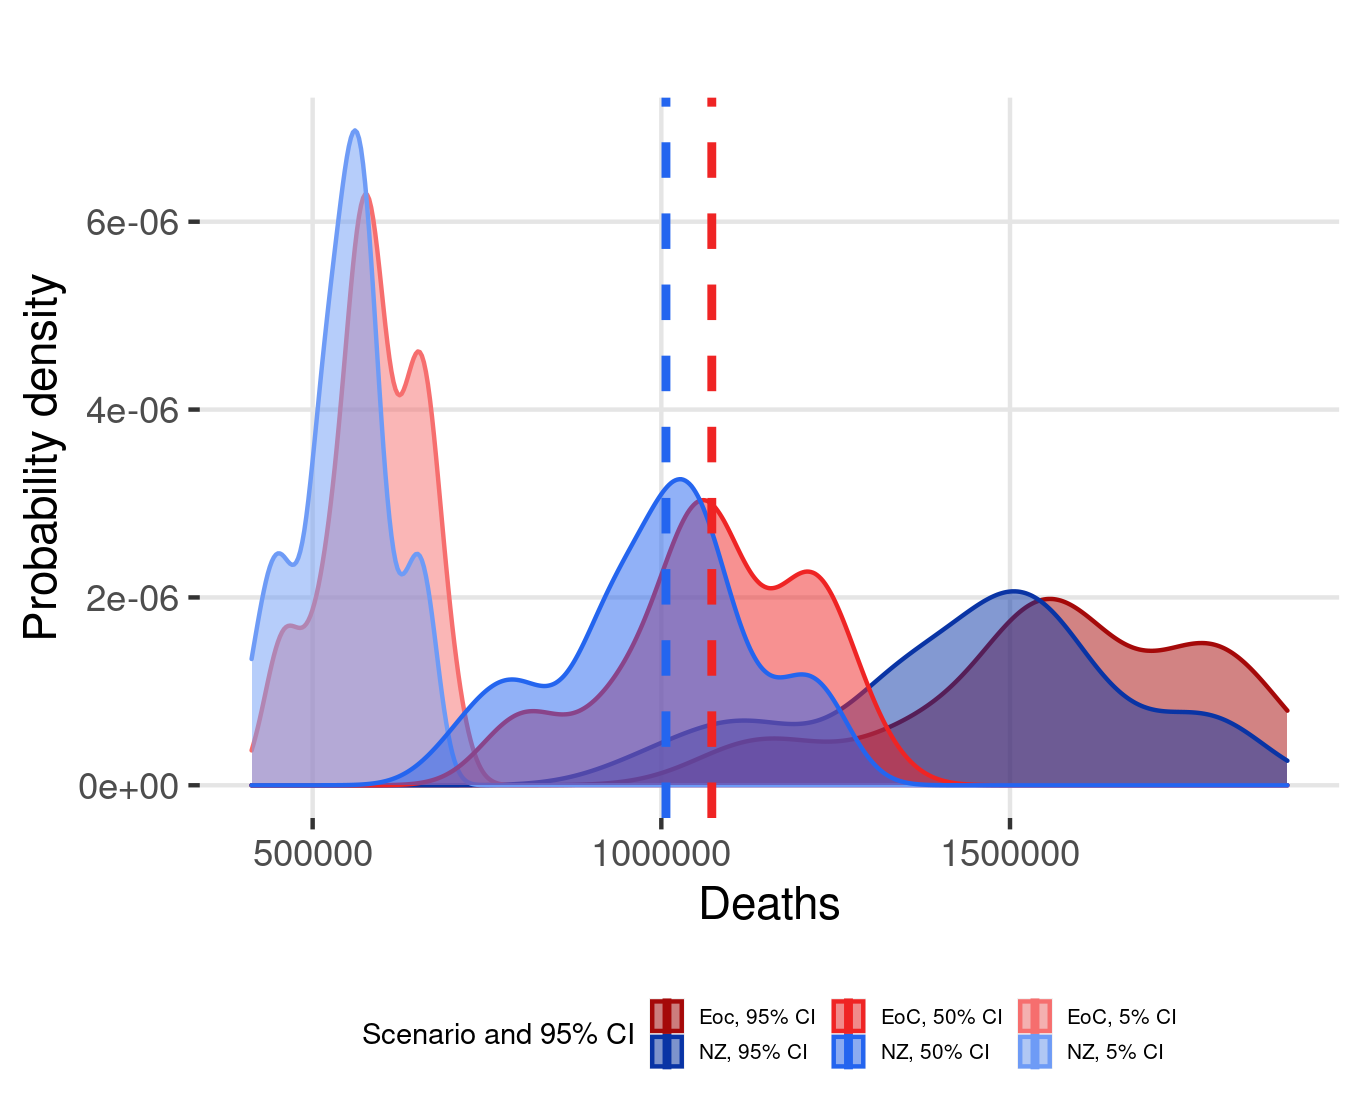
\includegraphics[width=2.7cm]{"Images_flow/plot_uncert_M.png"}};}
    \onslide<8-8>{\node[draw=red,rectangle,rounded corners,yshift = -0.5cm] (econUncert) [below = of econ] {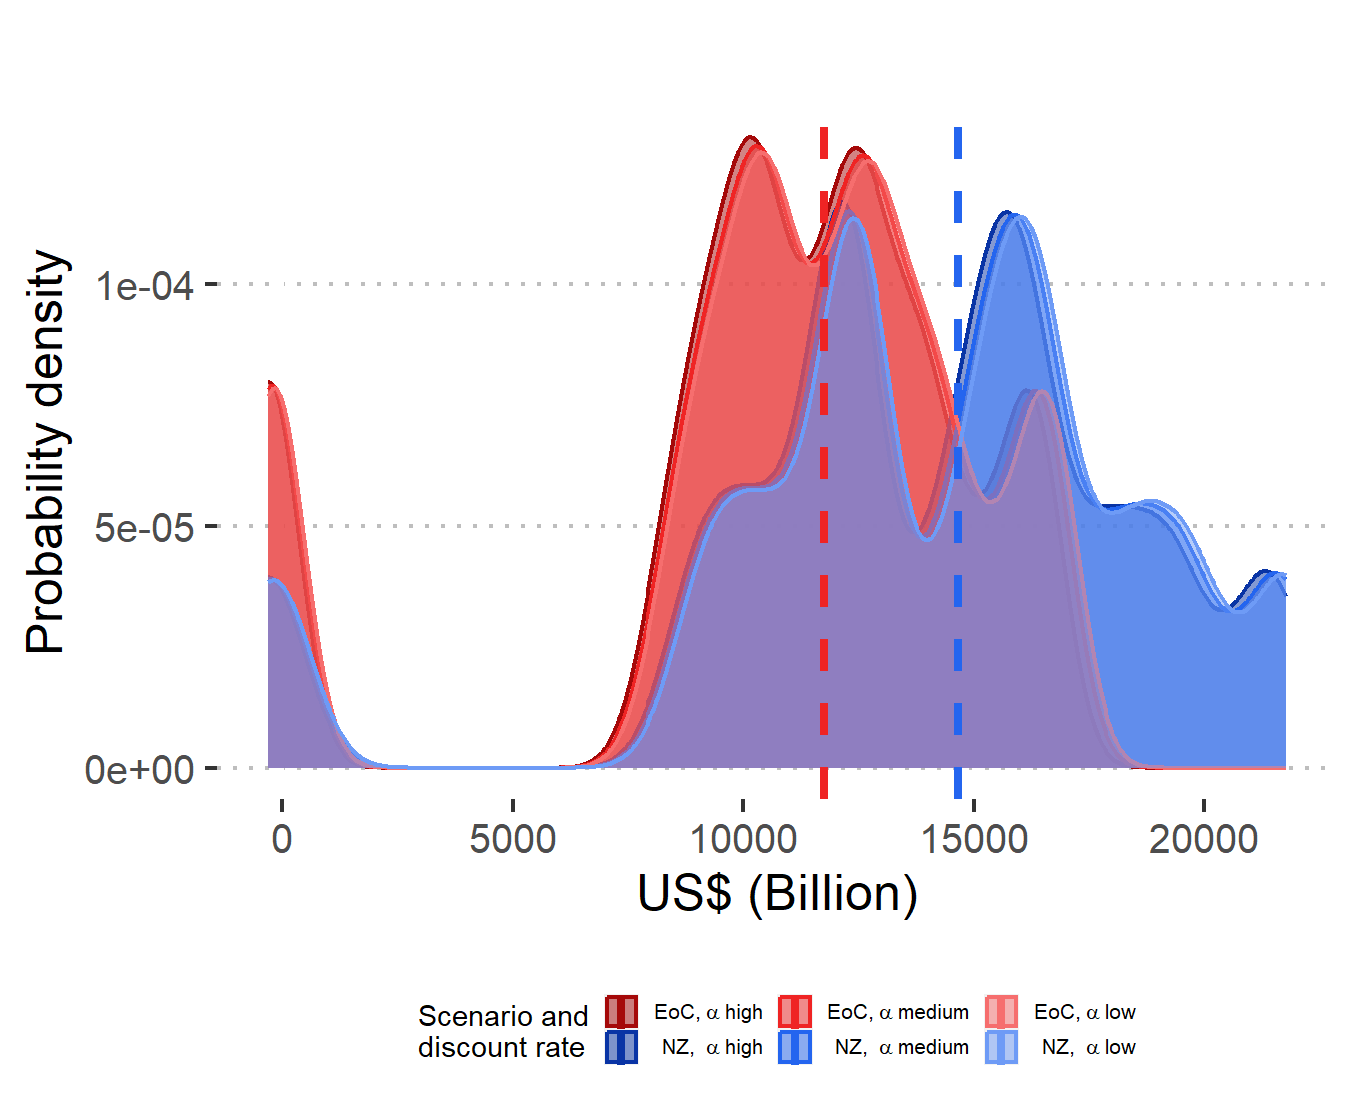
\includegraphics[width=2.7cm]{"Images_flow/plot_uncert_Econ.png"}};}

    \onslide<6-8>{\node[draw=red,ellipse,text width=3cm,align=center,text=red] (eng) {\tiny{Detailed database}};}
    \onslide<6-8>{\draw [->,red] (eng) to [out=180,in=130] node [text width=2.5cm,align=center,midway,above,red] {} (emi);}
    \onslide<6-8>{\draw [->,red] (emi) to [out=50,in=130] node [text width=2.5cm,align=center,midway,above,red] {\tiny{Chemical model}} (conc);}
    \onslide<6-8>{\draw [->,red] (conc) to [out=50,in=130] node [text width=2.5cm,align=center,midway,above,red] {\tiny{Impact functions}} (mort);}
    \onslide<6-8>{\draw [->,red] (mort) to [out=50,in=130] node [text width=2.5cm,align=center,midway,above,yshift=0.25cm] {\tiny{Econometric}} (econ);}
    \onslide<6-8>{\draw [->,red] (mort) to [out=50,in=130] node [text width=2.5cm,align=center,midway,above,xshift=0.25cm] {\tiny{equations}} (econ);}
    \onslide<6-8>{\draw [->,red] (1,-1.3) .. controls (2,-0.5) and (4,-0.5) .. (5,-1.3);}
  
    % Text
    \onslide<2-8>{\node (emiText) [above of=emi,text width=2cm,yshift=0.85cm,align=center,mypurple]{\tiny{Estimated emissions}};;}    
    \onslide<3-8>{\node (concText) [above of=conc,text width=3cm,yshift=0.85cm,align=center,mypurple]{\tiny{Computed concentrations}};;}    
    \onslide<4-8>{\node (mortText) [above of=mort,text width=2cm,yshift=0.85cm,align=center,mypurple]{\tiny{Health impact}};;}    
    \onslide<5-8>{\node (econText) [above of=econ,text width=2cm,yshift=0.85cm,align=center,mypurple]{\tiny{Economic impact}};;}

    % Arrows
    \onslide<2-6>{\draw [->,black] (eng) to [out=180,in=130] node [text width=2.5cm,align=center,midway,above] {} (emi);}

    \onslide<3-6>{\draw [->] (emi) to [out=50,in=130] node [text width=2.5cm,align=center,midway,above] {\tiny{Chemical model}} (conc);}
    \onslide<4-6>{\draw [->] (conc) to [out=50,in=130] node [text width=2cm,align=center,midway,above] {\tiny{Impact functions}} (mort);}    
    \onslide<5-6>{\draw [->] (mort) to [out=50,in=130] node [text width=2.5cm,align=center,midway,above,yshift=0.25cm] {\tiny{Econometric}} (econ);}
    \onslide<5-6>{\draw [->] (mort) to [out=50,in=130] node [text width=2.5cm,align=center,midway,above,xshift=0.25cm] {\tiny{equations}} (econ);}
    \onslide<5-6>{\draw [->] (1,-1.3) .. controls (2,-0.5) and (4,-0.5) .. (5,-1.3);}
    
    \onslide<8-8>{\draw [->,dotted,black] (emi) to [out=270,in=90] node [text width=2.5cm,align=center,midway,above] {} (emiUncert);}
    \onslide<8-8>{\draw [->,dotted,black] (conc) to [out=270,in=90] node [text width=2.5cm,align=center,midway,above] {} (concUncert);}
    \onslide<8-8>{\draw [->,dotted,black] (mort) to [out=270,in=90] node [text width=2.5cm,align=center,midway,above] {} (mortUncert);}
    \onslide<8-8>{\draw [->,dotted,black] (econ) to [out=270,in=90] node [text width=2.5cm,align=center,midway,above] {} (econUncert);}

\end{tikzpicture}

\end{center}
\end{frame}




